%-*-coding: utf-8-*-
\chapter{Практическая реализация и результаты}

\label{ch:implementation}

В данной главе рассмотрены некоторые аспекты практической реализации
предложенного алгоритма и визуализации. Программный модуль, решающий
поставленную задачу, был реализован на языке C++ в рамках имеющегося
фреймворка для решения задач. В заключение приводятся основные
результаты работы.

\FloatBarrier

\section{Предобработка}

\label{sec:preprocessing-impl}

Для решения большей части задач по предобработке данных использованы
библиотеки ЗАО «Кронштадт Технологии». Чтение исходных данных и
классификация объектов карты осуществляется с помощью имеющихся утилит
импорта картографических данных. Для выполнения геометрических
операций, таких как объединение контуров, упрощение полилиний,
построение straight skeleton, смещение полигона и т. д., используется
библиотека геометрических примитивов и алгоритмов ЗАО «Кронштадт
Технологии». Также в этой библиотеке есть специальная структура
данных, названная \emph{Contours Set}, для эффективной проверки
пересечения отрезка с полигоном. Эта структура данных активно
используется для всех проверок корректности рёбер (при добавлении
рёбер, сглаживании маршрута, упрощении цепочек рёбер straight
skeleton'а).

\begin{figure}
    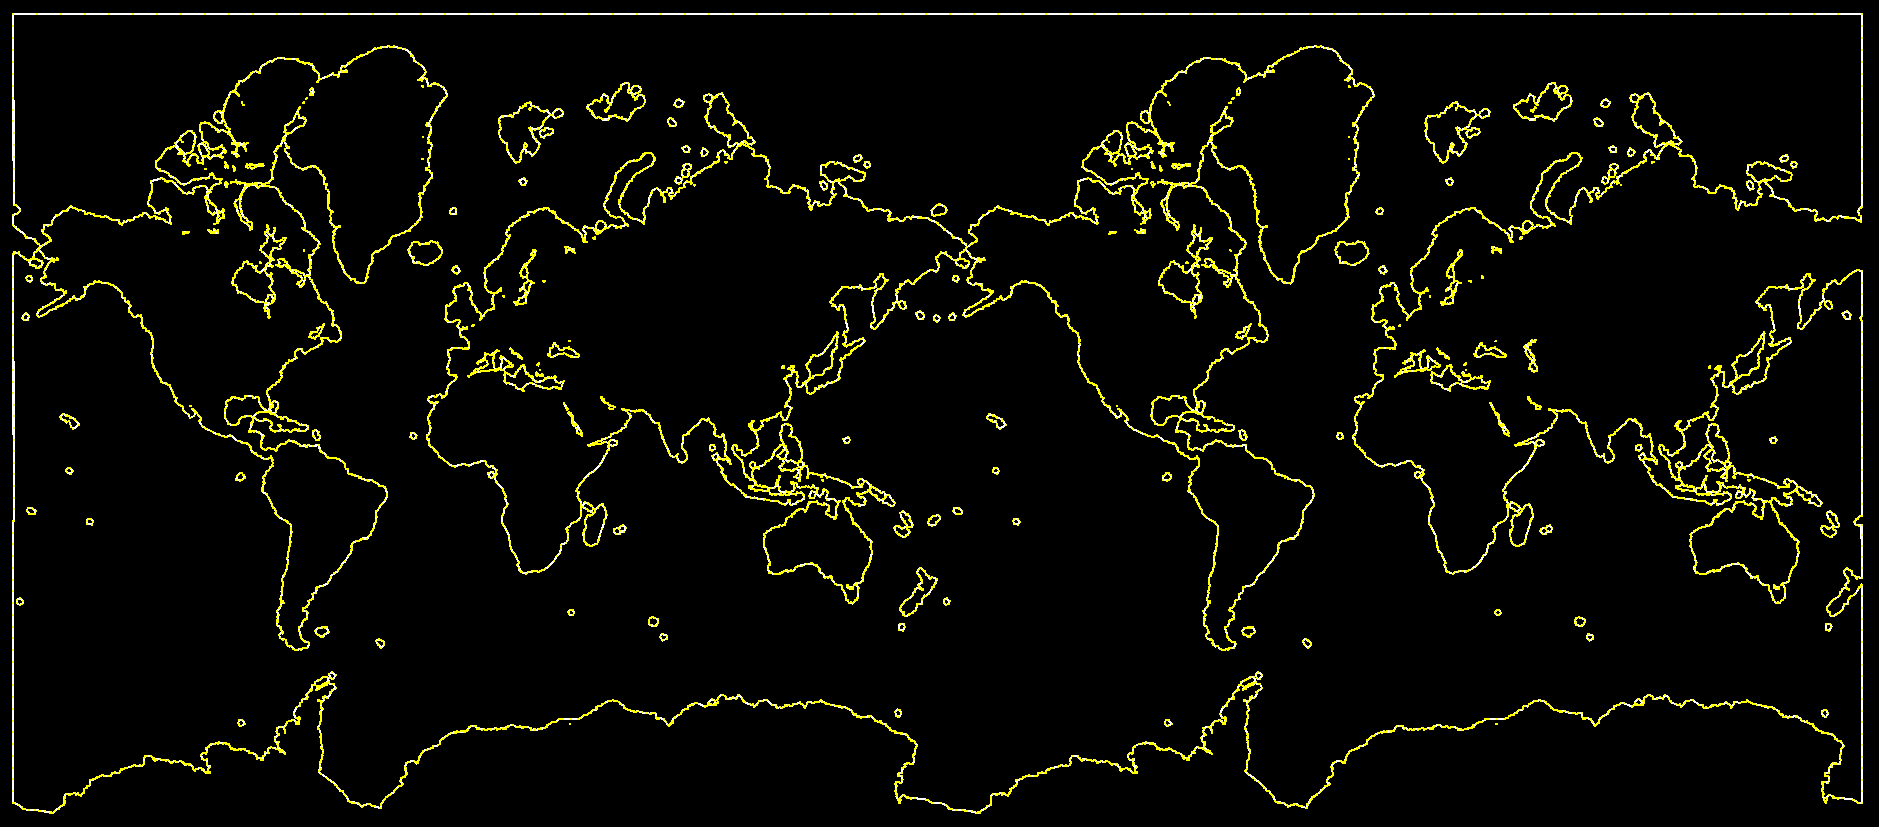
\includegraphics[width=\textwidth]{Solution/doubled-offseted-polygon}
    \caption{Полигон, объединённый со смещённой копией}
    \label{fig:doubled-polygon}
\end{figure}

Определённую сложность представляет добавление рёбер через 180-ый
меридиан. Для этого имеющийся полигон, ограничивающий воду,
объединяется со своей копией, сдвинутой влево на длину плоскости
проекции. В результате получается полигон, изображённый на
рисунке~\ref{fig:doubled-polygon}. По такому полигону можно легко
проверять корректность ребра, проходящего через 180-ый меридиан,
переместив его восточную точку влево на длину плоскости проекции.

Для тестирования работы алгоритма использовались свободно
распространняемые данные OpenStreetMap~\cite{osm}. Получившийся граф
содержит 13344 вершины и 124324 ребра.

\FloatBarrier

\section{Вычисление метрик}

\label{sec:metrics-computation}

Поскольку в процессе работы алгоритма для всех пар путей проверяется
критерий похожести, необходимо добиться высокой скорости вычисления
метрик на маршрутах. Для вычисления обеих метрик используются длины
кратчайших расстояний между парами вершин в графе. Длины кратчайших
расстояний между всеми парами вершин могут быть найдены с помощью
алгоритма Флойда~\cite{floyd1962algorithm}. Однако алгоритм Флойда
работает за время порядка $\Theta(n^3)$, что неприемлимо для графа,
содержащего 13344 вершины. Также нетрудно заметить, что знать длины
кратчайших путей в графе между всеми парами вершин не нужно, поскольку
в определении обеих метрик присутствуют лишь длины кратчайших путей
для всех пар вершин, принадлежащих первому и второму маршруту. Поэтому
можно для каждой вершины первого пути использовать алгоритм Дейкстры и
останавливать поиск при достижении какой-либо вершины второго пути.
Поскольку в этом случае время работы сильно зависит от конкретных
маршрутов (не только от числа вершин, но и от их расположения,
поскольку каждый поиск алгоритмом Дейкстры может заканчиваться очень
рано или, наоборот, спустя большое число итераций), то теоретические
оценки времени работы такого подхода не несут практической информации.
На практике же при таком способе вычисления метрик поиск маршрутов,
как правило, занимал 2--10 секунд. Однако поставленная задача требует
выполнять запросы за время, не превышающее одной секунды.

Для улучшения производительности было сделано две оптимизации.
Нетрудно заметить, что если в процессе вычисления первой метрики
находится пара вершин из первого и второго маршрута, между которыми
длина кратчайшего пути в графе больше порогового значения, то можно
заключить, что маршруты непохожи. При вычислении второй метрики верен
аналогичный факт. Таким образом, поскольку метрики считаются только
для проверки критерия похожести маршрутов, то вычисление можно
останавливать, как только найдена пара вершин, гарантирующая
непохожесть маршрутов.

Вторая оптимизация затрагивает сам процесс вычисления метрик. Вместо
поиска кратчайших расстояний с помощью алгоритма Дейкстры из всех
вершин пути используется другой подход. Сначала строится граф с
фиктивной вершиной~($f$), из которой проведены рёбра нулевого веса во
все вершины первого маршрута~($P$). Затем с помощью алгоритма Дейкстры
находятся длины кратчайших расстояний из фиктивной вершины до всех
вершин второго маршрута~($Q$) (поиск заканчивается, когда посещены все
вершины, принадлежащие $Q$). Поскольку из фиктивной вершины проведены
рёбра нулевого веса во все вершины, принадлежащие $P$, и только в них,
то кратчайший путь от неё до вершины $v \in Q$ будет иметь вид
$fu \dots v$ для какой-то вершины $u \in P$, и его длина будет равна
$\rho_g(u, v)$. Как и в определении метрик за $\rho_g(u, v)$
обозначена длина кратчайшего пути между вершинами $u$ и $v$ в графе.
Нетрудно заметить, что в этом случае
$\rho_g(u, v) = \min\limits_{w \in P} \rho_g(w, v)$. Действительно,
пусть существует вершина $u' \in P$, такая что
$\rho_g(u', v) < \rho_g(u, v)$. Обозначим кратчайший путь в графе
между $u'$ и $v$ как $R = u'r_0r_1 \dots r_nv$. Тогда длина пути
$fu'r_0 \dots r_nv$ равна
$\rho_g(u', v) < \rho_g(u, v) = \rho_g(f, v)$, что противоречит тому,
что $\rho_g(f, v)$ является длиной кратчайшего пути из $f$ в $v$.
Значит, предположение о существовании $u'$ неверно. Таким образом,
сразу для всех вершин $v \in Q$ находится величина
$\min\limits_{u \in P} \rho_(u, v)$ за один обход алгоритма Дейкстры.
Аналогичный поиск можно выполнить, добавив фиктивную вершину и рёбра
нулевого веса во все вершины маршрута $Q$, тем самым найдя для всех
$u \in P$ величину $\min\limits_{v \in Q} \rho_(u, v)$. После этого
достаточно взять максимум всех найденных величин, который будет
значением метрики. При этом, как было сказано ранее, если хоть одно из
найденных значений больше определённого порога (описанного в критерии
похожести), то вычисление можно сразу же закончить, заключив, что
маршруты непохожи. Для вычисления второй метрики помимо максимального
минимального расстояния между парами вершин нужно находить расстояние
до ближайшей вершины в мире. Данный поиск был реализован простым
перебором, работающим в худшем случае за время порядка
$\Theta(l1 \cdot l2)$, где $l1$ и $l2$ --- длины первого и второго
маршрута соответственно. Однако, во-первых, вторая метрика
вычисляется, как правило, реже, чем первая, во-вторых, зачастую не
нужно просматривать все вершины, поскольку пара вершин, для которых
выполнен критерий непохожести, встречается раньше. Помимо этого при
вычислении второй метрики не рассматриваются пары вершин, ребро между
которыми не пересекает ни одно препятствие, поскольку между такими
вершинами можно пройти по прямой. В результате проведённых оптимизаций
время обработки запроса существенно уменьшилось и стало составлять
порядка 0,2--0,8 секунды. При этом профилирование показало, что
основную часть времени стало занимать не вычисление метрик, а
сокращение маршрутов. Поскольку итоговое время работы удовлетворяет
поставленным требованиям, дальнейшие оптимизации не проводились.

\FloatBarrier

\section{Запретные зоны}

\label{sec:forbidden-zones}

Помимо поиска маршрутов по имеющейся карте, важно предоставить
пользователю возможность самостоятельно добавлять и удалять запретные
зоны, которые являются дополнительными полигональными препятствиями.
Во-первых, в реальной жизни действительно в различных регионах может
быть запрещено проплыть (например, из-за военных учений). Во-вторых,
за счёт этого пользователь может влиять на семейство находимых
маршрутов, например, запрещать маршрут, который по тем или иным
причинам не подходит. Такая важная функциональность, однако,
реализуется очень просто. Для этого используется обёртка над графом,
хранящая уже упомянутую структуру \emph{Contours Set} с запретными
зонами. При запросе рёбер они фильтруются по предикату, проверяющему,
что ребро не пересекает запретные контура. Нетрудно заметить, что для
предложенного алгоритма такие запретные зоны, по сути, ничем не
отличаются от исходных полигональных препятствий, поскольку они просто
запрещают определённые рёбра в графе. Таким образом, способ обхода
запретных зон также будет влиять на похожесть маршрутов. На
рисунке~\ref{fig:forbidden} представлен пример маршрутов при наличии
запретной зоны.

\begin{figure}
    \begin{center}
        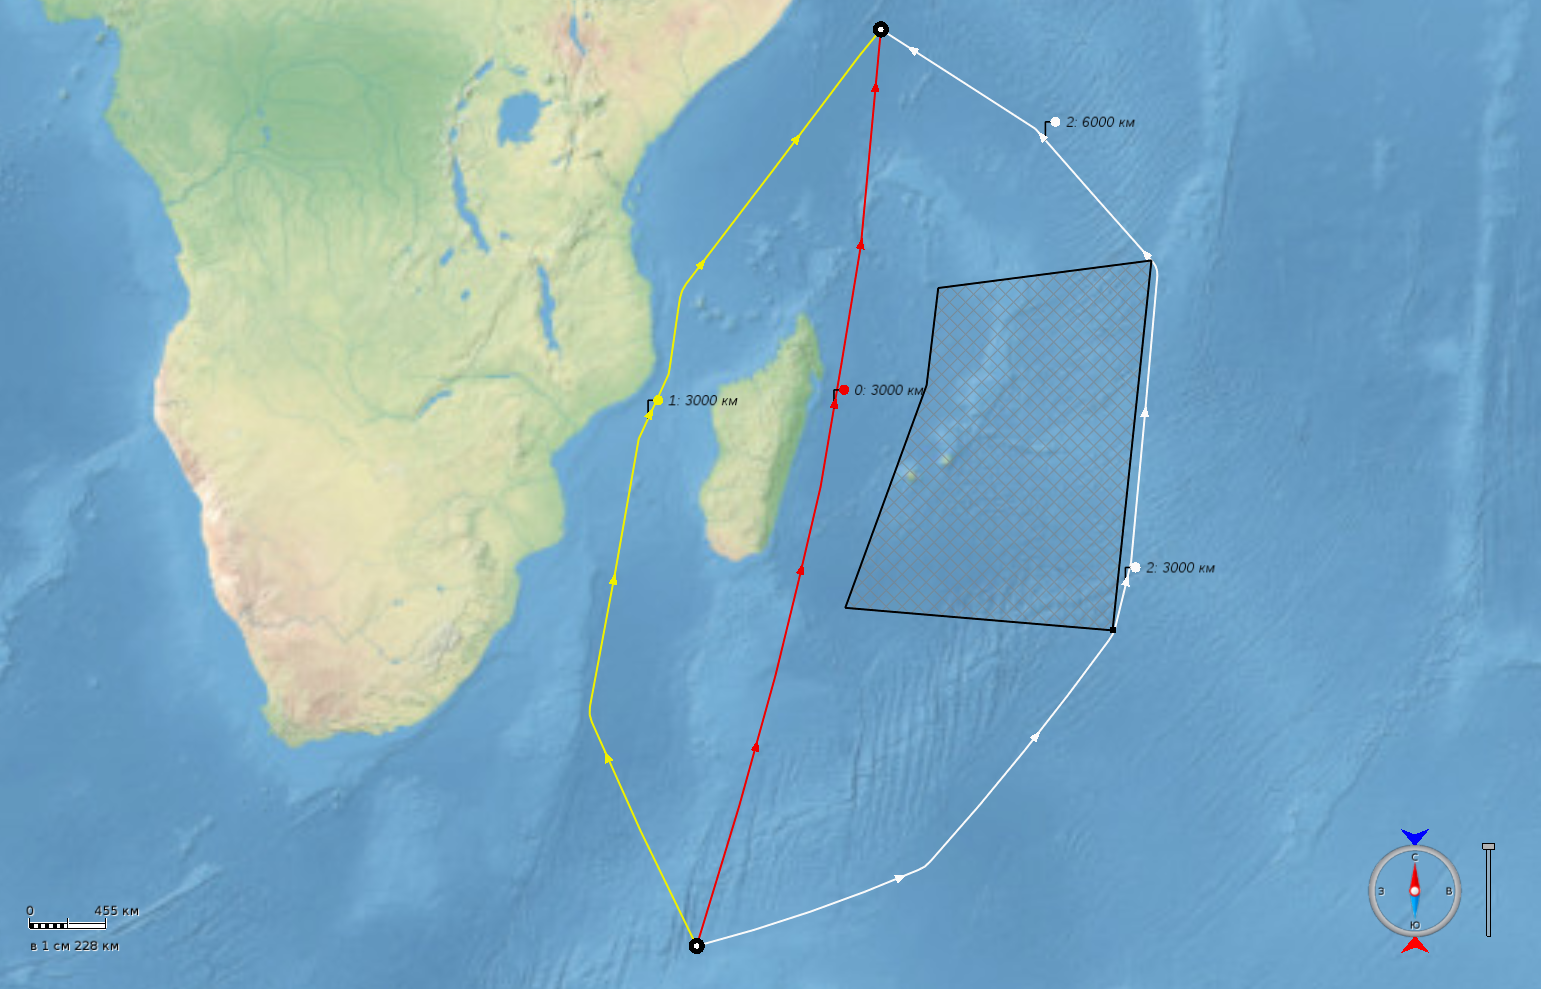
\includegraphics[width=.85\textwidth, clip=true, trim = 0pt 0pt
        250pt 0pt]{Solution/forbidden-zones}
    \end{center}
    \caption{Маршруты при наличии запретной зоны}
    \label{fig:forbidden}
\end{figure}

\FloatBarrier

\section{Визуализация}

\label{sec:visualization-impl}

Для визуализации маршрутов была использована библиотека, разработанная в
ЗАО~«Кронштадт Технологии» и основанная на OpenGL~\cite{opengl}. Данная
библиотека позволяет отображать различные примитивы на плоскости и
сфере, в том числе полилинии на сфере. Основная проблема при
визуализации семейств маршрутов состоит в том, что некоторые маршруты
накладываются друг на друга. Решение такой проблемы состоит в смещении
перекрывающихся частей на небольшое расстояние в пикселях. Для этого
выделяются перекрывающиеся части имеющихся маршрутов (имеющие
одинаковые рёбра) с помощью сохранения рёбер в хеш-таблицу. При
визуализации каждое ребро маршрута рассматривается отдельно. Если оно
принадлежит более чем одному маршруту, то берётся порядковый номер
текущего пути в отсортированном списке маршрутов, содержащих данное
ребро, и вычисляется величина смещения путём домножения этого номера
на текущий размер пикселя в мире. Затем каждая вершина ребра смещается
на эту величину в направлении бисектрисы, проведённой в треугольнике,
образованном текущей вершиной и её соседними вершинами. Если одной из
соседних вершин не существует (вершина является начальной или конечной
точкой), то в качестве направления берётся нормаль к соответствующему
ребру. В следующем разделе приведены рисунки с примерами работы
алгоритма, на которых можно видеть смещённые маршруты.

\FloatBarrier

\section{Результаты}

\label{sec:results}

По итогам данной работы получены следующие результаты:
\begin{itemize}
    \item Исследованы имеющиеся подходы к решению аналогичных задач,
      выявлены и продемонстрированы их недостатки.
    \item Сформулировано формальное описание поставленной задачи.
    \item Предложены алгоритмы и эвристики для решения поставленной
      задачи.
    \item Реализован программный модуль, решающий поставленную задачу.
    \item Получено заключение экспертов ЗАО~«ОСК-Транзас» о том, что
      находимые маршруты удовлетворяют поставленным требованиям.
      Эвристики, разработанные для поиска различных маршрутов,
      признаны эффективными и разумными. Алгоритм и критерии,
      заложенные в программный модуль, рекомендованы для решения задач
      поддержки принятия решения в навигационно-тактических системах
      морского назначения.
    \item Разработанный программный модуль внедрён в имеющийся
      3D-клиент ЗАО~«Кронштадт Технологии».
\end{itemize}

\begin{figure}
    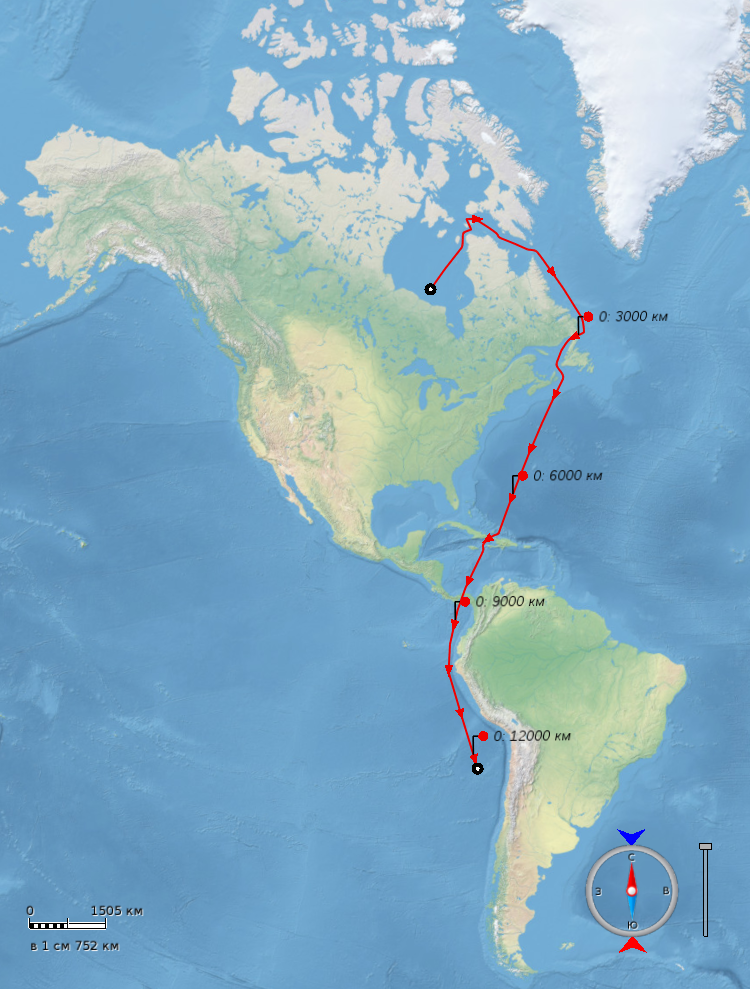
\includegraphics[width=\textwidth]{Results/comparison/bad1}
    \caption{Найден лишь один маршрут}
    \label{fig:res-comp-bad1}
\end{figure}

\begin{figure}
    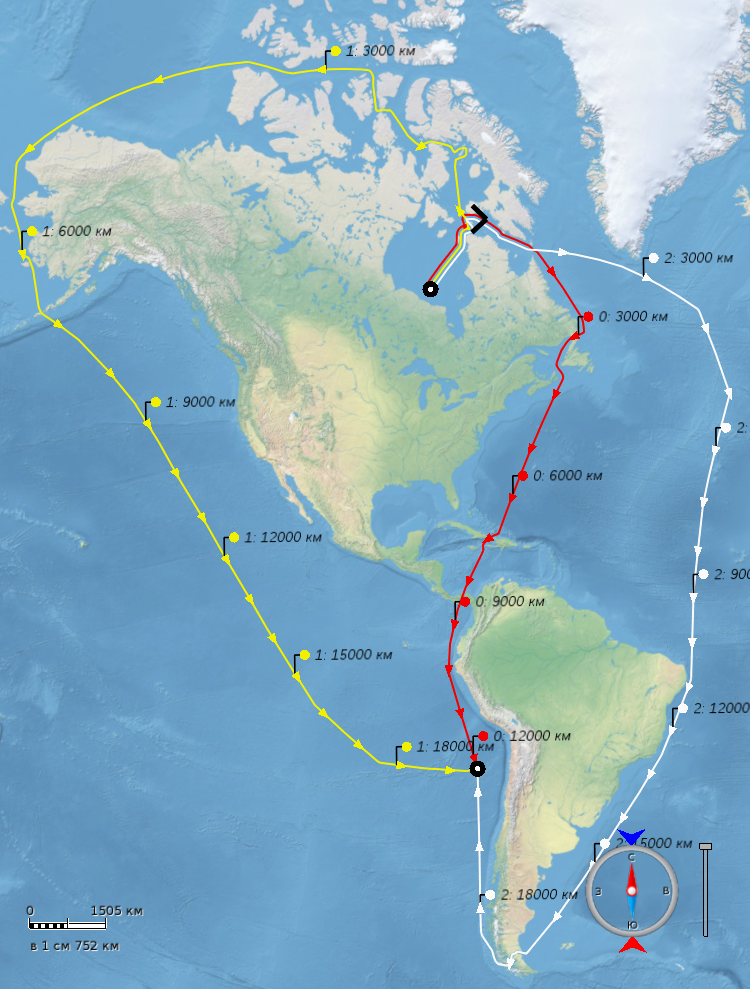
\includegraphics[width=\textwidth]{Results/comparison/good1}
    \caption{Найдено три различных маршрута}
    \label{fig:res-comp-good1}
\end{figure}

\begin{figure}
    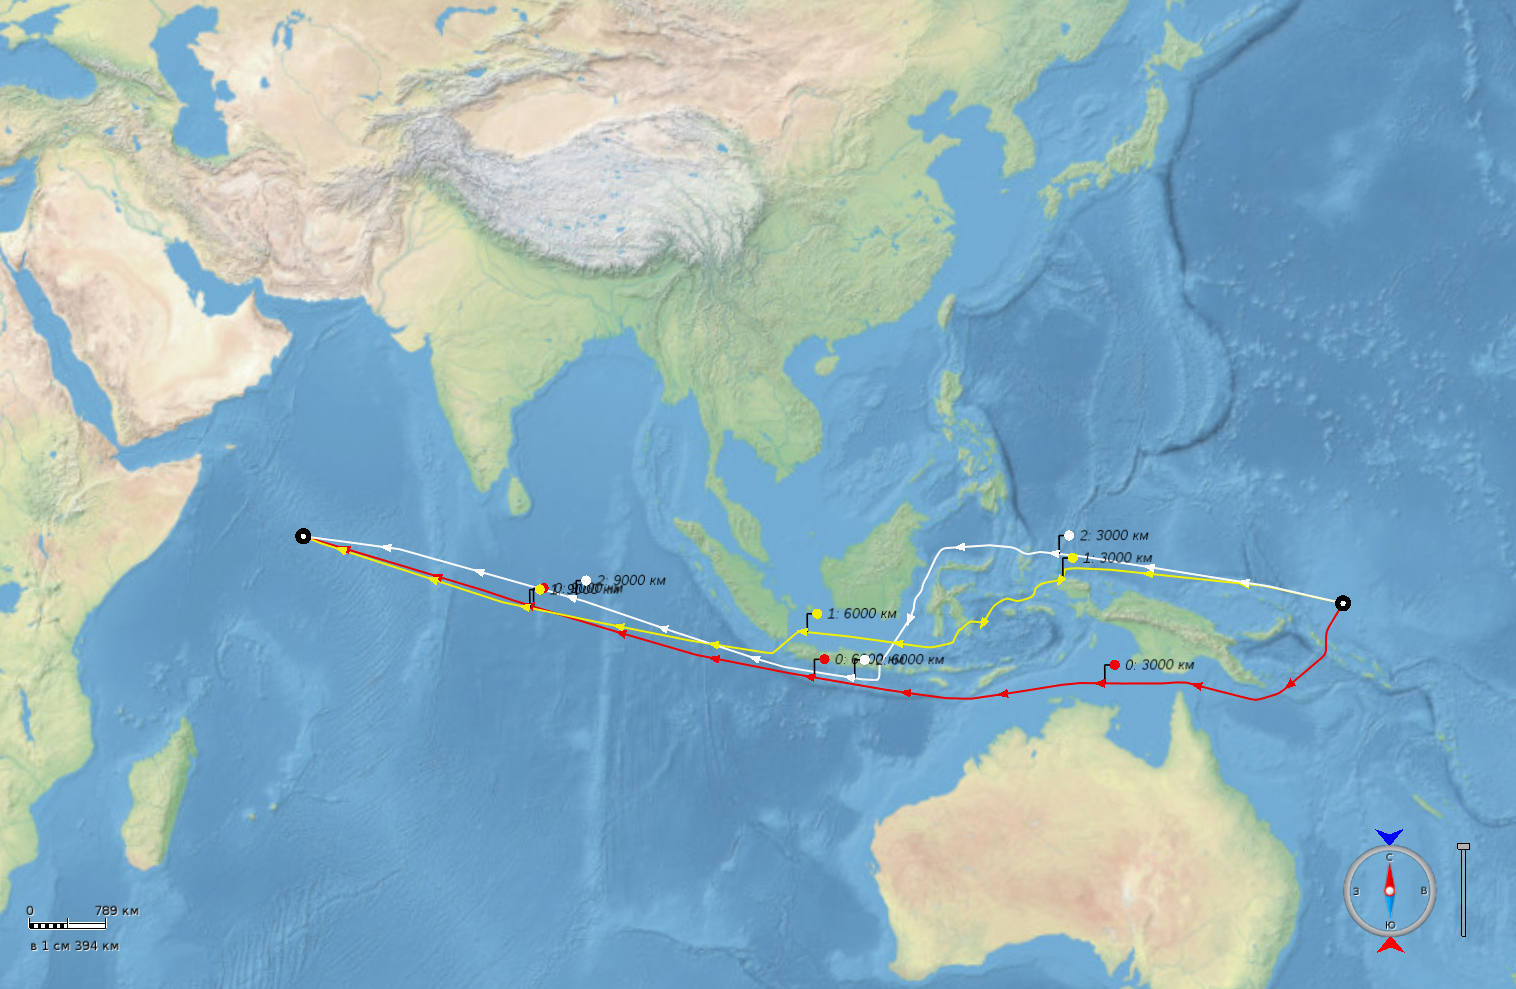
\includegraphics[width=\textwidth]{Results/comparison/bad2}
    \caption{Найдены похожие маршруты}
    \label{fig:res-comp-bad2}
\end{figure}

\begin{figure}
    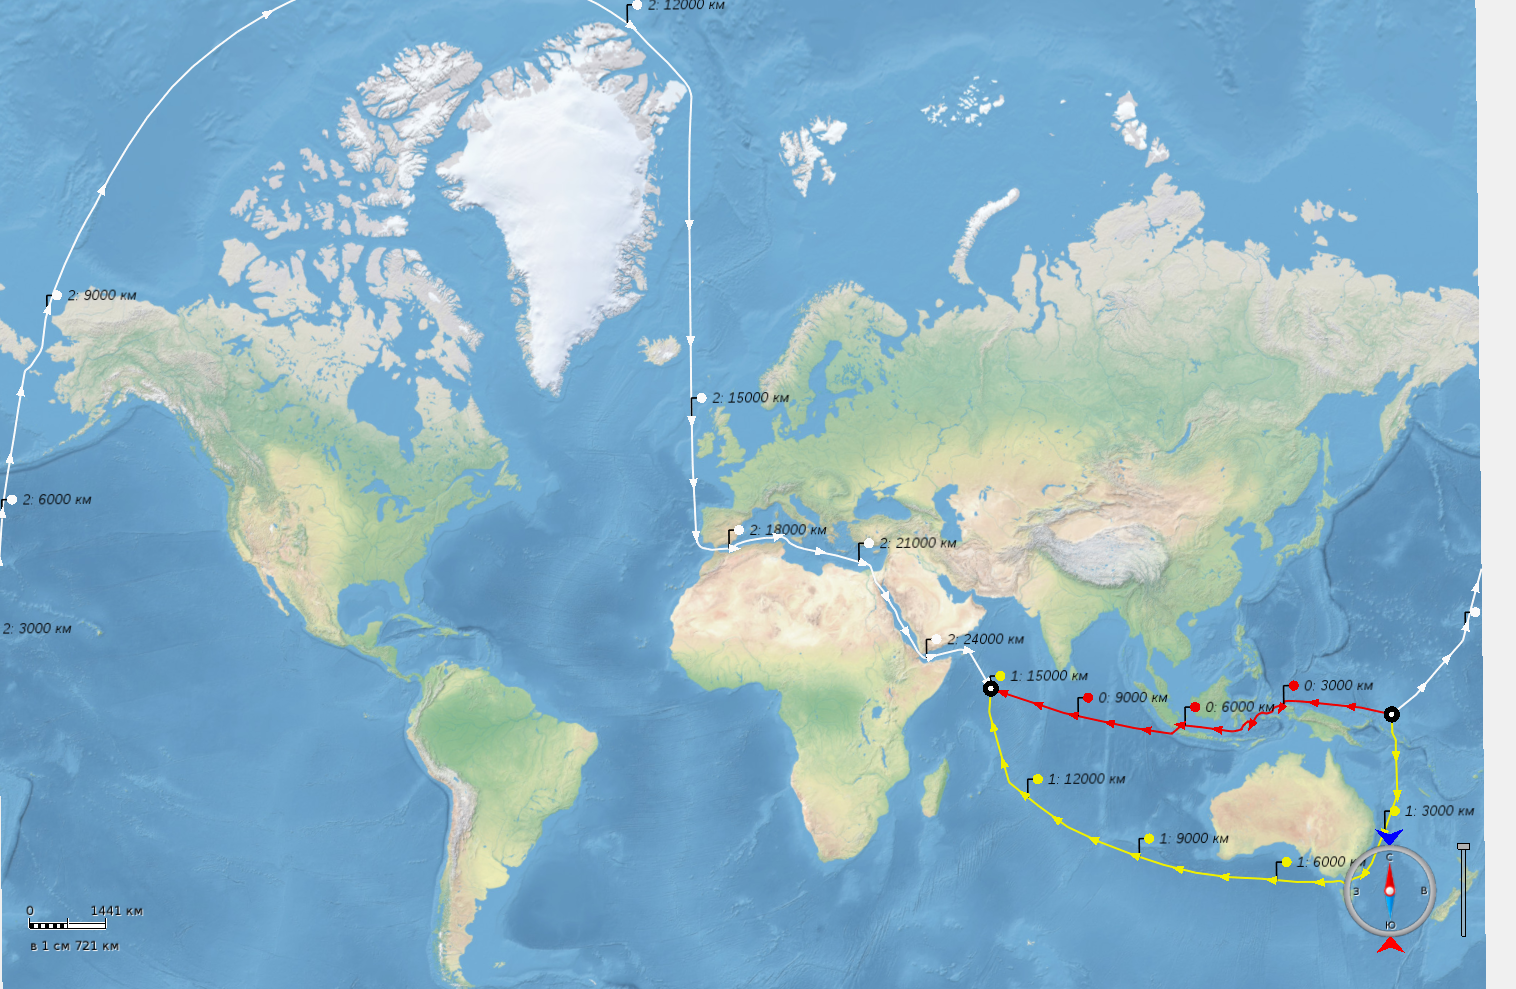
\includegraphics[width=\textwidth]{Results/comparison/good2}
    \caption{Найдены маршруты с разными способами обхода материков}
    \label{fig:res-comp-good2}
\end{figure}

Для примера проведём сравнение маршрутов, находимых разработанным
алгоритмом, с маршрутами, находимыми
алгоритмом~\cite{lim2005shortest}. На рисунках \ref{fig:res-comp-bad1}
и \ref{fig:res-comp-good1} показана ситуация, в которой алгоритм,
описанный Лимом и Кимом, нашёл лишь один маршрут, а алгоритм,
описанный в данной работе, нашёл три различных маршрута. В ситуации,
показанной на рисунках \ref{fig:res-comp-bad2} и
\ref{fig:res-comp-good2}, оба алгоритма нашли три маршрута. Однако в
первом случае маршруты, не являются существенно различными, хоть и
обходят препятствия разными способами, поскольку размеры этих
препятствий невелики. К тому же найденные маршруты не являются
локально оптимальными, так как в конце пути имеются некоторые
различия. Во втором случае было найдено три существенно разных
маршрута, различающихся способами обхода материков. Таким образом,
показано, что разработанный алгоритм лучше подходит для решения
поставленной задачи, хотя общая идея у них похожа.

В заключение приведём несколько рисунков, демонстрирующих результаты
работы алгоритма на сфере (рис.~\ref{fig:result1}, \ref{fig:result2}).

\begin{figure}
    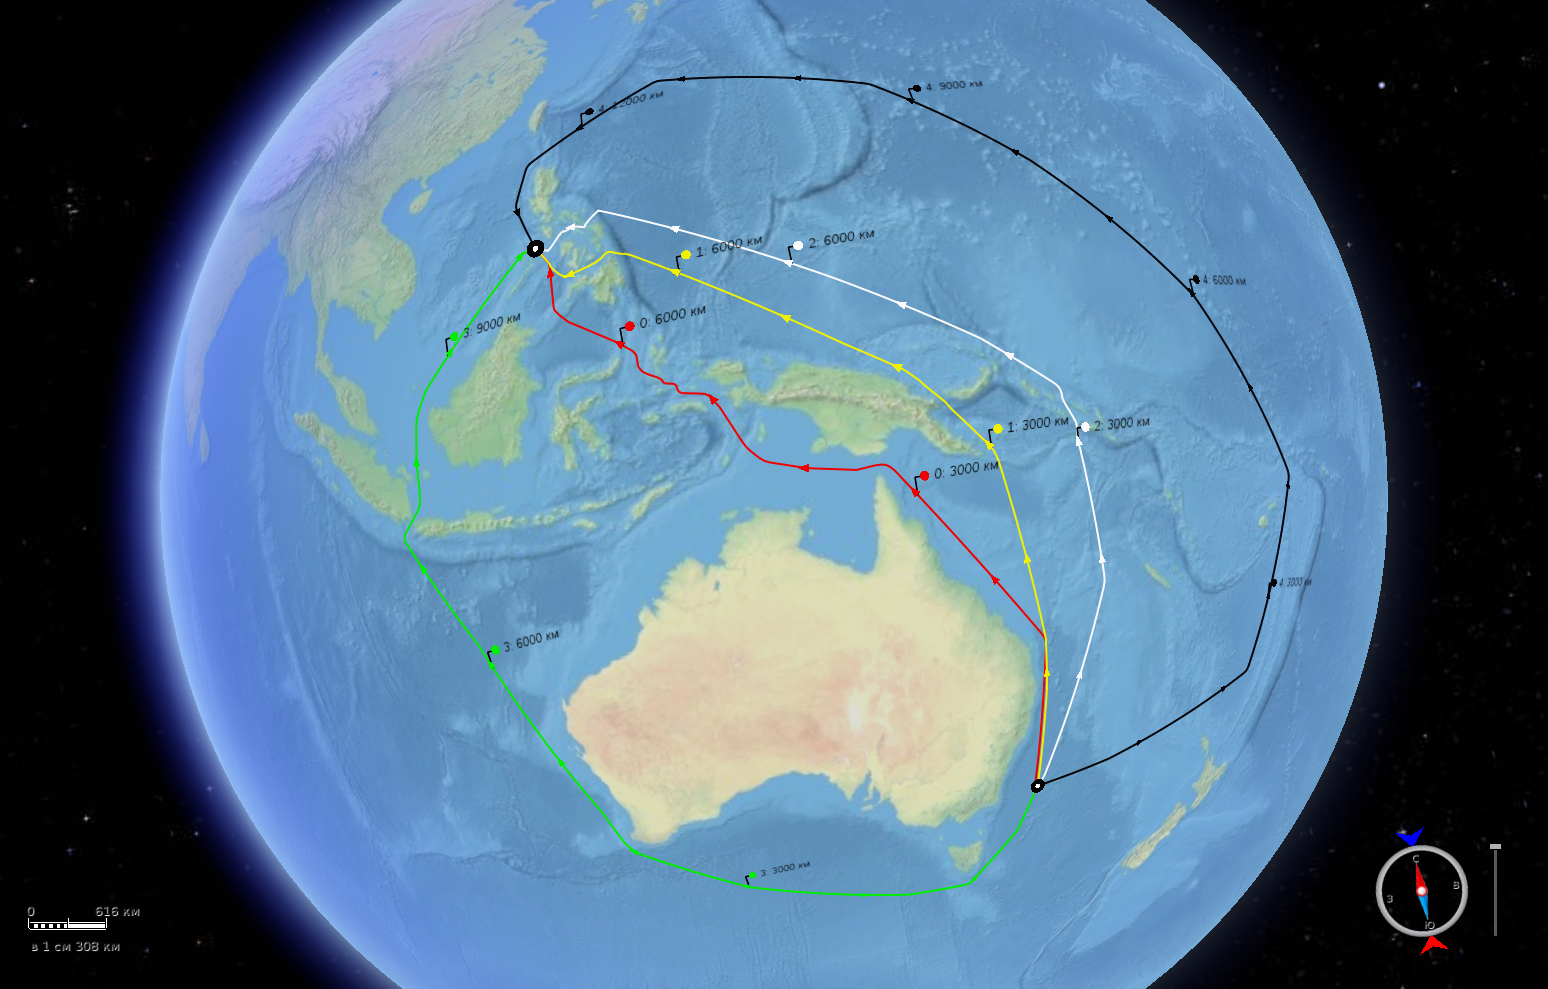
\includegraphics[width=\textwidth]{Results/1}
    \caption{Маршруты на сфере}
    \label{fig:result1}
\end{figure}

\begin{figure}
    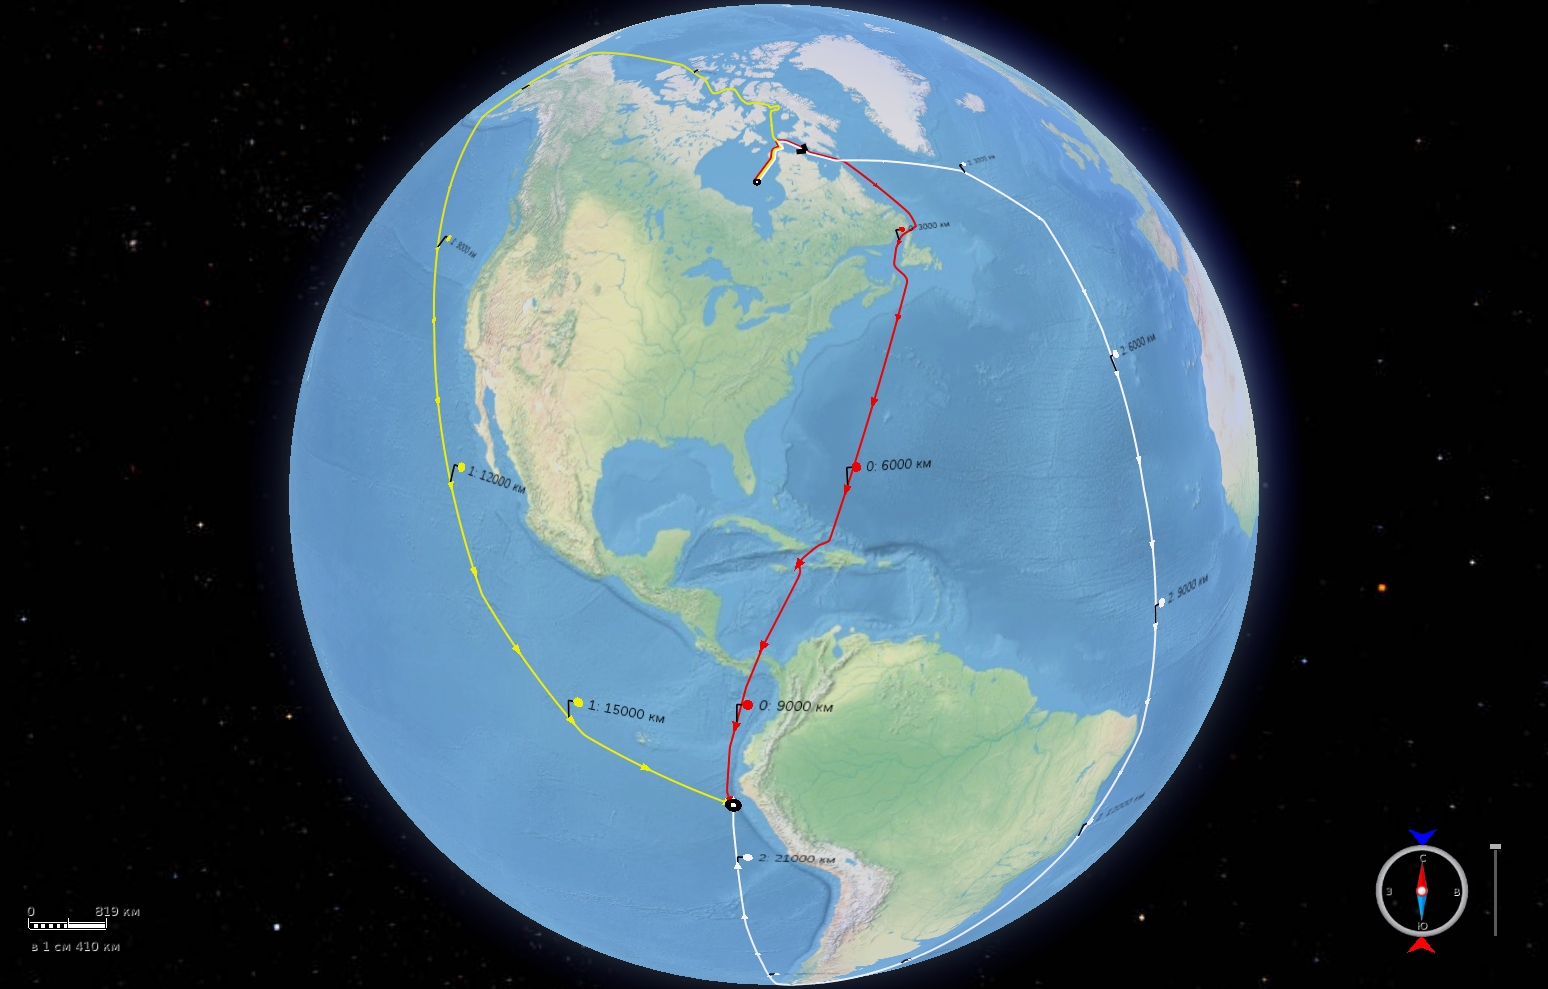
\includegraphics[width=\textwidth]{Results/2}
    \caption{Маршруты на сфере}
    \label{fig:result2}
\end{figure}

\FloatBarrier

